% Source of the journal-format manuscript (Izvestiya RAN, Ser. Geogr., rules of 17.11.2025).
% Citation placeholders and the two bibliography markers are expanded by
% tools/build_article1_journal.py into article1_v7.tex (plain-text author-year citations).
\documentclass[12pt,a4paper]{article}
\usepackage[a4paper,top=2cm,bottom=2cm,left=3cm,right=1.5cm]{geometry}
\usepackage{iftex}
\ifPDFTeX
  \usepackage[T2A]{fontenc}
  \usepackage[utf8]{inputenc}
  \usepackage[russian]{babel}
\else
  \usepackage{fontspec}
  \usepackage{polyglossia}
  \setdefaultlanguage{russian}
  \setotherlanguage{english}
  \defaultfontfeatures{Ligatures=TeX}
  \IfFontExistsTF{Times New Roman}{%
    \setmainfont{Times New Roman}\newfontfamily\cyrillicfont{Times New Roman}%
  }{%
    \IfFontExistsTF{Liberation Serif}{%
      \setmainfont{Liberation Serif}\newfontfamily\cyrillicfont{Liberation Serif}%
    }{\setmainfont{CMU Serif}\newfontfamily\cyrillicfont{CMU Serif}}%
  }
\fi
\usepackage{setspace}
\usepackage{mathtools,amssymb}
\usepackage{graphicx}
\usepackage{booktabs}
\usepackage{array}
\usepackage{caption}
\captionsetup{labelsep=period,font=normalsize,justification=raggedright,singlelinecheck=false}
\usepackage{titlesec}
\titleformat{\section}{\normalfont\bfseries\centering}{}{0pt}{}
\titleformat{\subsection}{\normalfont\itshape}{}{0pt}{}
\titlespacing*{\section}{0pt}{18pt}{6pt}
\titlespacing*{\subsection}{0pt}{12pt}{3pt}
\usepackage[unicode,hidelinks]{hyperref}
\setlength{\parindent}{1.25cm}
\setlength{\emergencystretch}{3em}
\hyphenpenalty=10000 \exhyphenpenalty=10000
\onehalfspacing
\pagestyle{plain}

\newcommand{\Psurr}{P_{\mathrm{surr}}}

\begin{document}

\noindent УДК 551.513

\begin{center}
{\large\bfseries Сопряженность иерархических уровней атмосферной циркуляции как региональный инвариант}

\medskip
{\bfseries Н. С. Сотириади\textsuperscript{*}}

Независимый исследователь, [город], Россия

\textsuperscript{*}E-mail: n.sotiriadi@gmail.com
\end{center}

\begin{singlespace}
\noindent\textbf{Аннотация.} Спектральный и фрактальный анализ географических полей отвечает на вопрос, на каких масштабах располагаются уровни организации геосистемы. Следующий вопрос касается отношения между уровнями: предопределено ли размещение мезомасштабной изменчивости соседним крупным уровнем или она размещается по собственным локальным причинам. По полю относительного вихря на поверхности 850 гПа (реанализ ERA5, 2017--2024 гг.; 12 основных и 27 контрольных областей) построена мера такого отношения -- профиль сопряженности соседних октавных уровней $P$: пространственная корреляция карт активности двух соседних масштабов, очищенная от вклада самой процедуры разложения. Проверена гипотеза о том, что профиль является региональным инвариантом в операциональном смысле: сохраняет значение при смене сезона, года, фазы Эль-Ниньо -- Южного колебания, источника данных и схемы разбиения территории, различая при этом циркуляционные режимы. Гипотеза подтверждена на выборках, не участвовавших в построении величины ($p = 0.001$). Четыре альтернативных объяснения -- численная диссипация реанализа, спектр мощности поля, геометрия градусной сетки и устройство наблюдательной сети -- проверены прямыми контролями: региональная сигнатура сохраняется при ограничении разрешенными ступенями, содержит воспроизводимую информацию сверх спектра (контроль равновеликими областями: $p = 0.033$), воспроизводится при равновеликой нарезке территории и в свободном модельном расчете без усвоения атмосферных наблюдений (ранговая корреляция 0.71 при внутреннем пределе метода 0.93). Более высокие значения свойственны внетропическим штормовым путям, более низкие -- влажно-конвективным режимам; бассейны Конго и Амазонии при сходных стандартных характеристиках режима различаются архитектурой иерархии. Величина дополняет аппарат районирования характеристикой устройства межуровневых связей; границы ее применимости, включая отвергнутые интерпретации, перечислены явно.

\smallskip
\noindent\textbf{Ключевые слова:} иерархическая организация геосистем, инварианты динамической геосистемы, масштаб, мезомасштабная изменчивость, штормовые пути, глубокая конвекция, реанализ, районирование, фальсификационная схема.
\end{singlespace}

\section{ПОСТАНОВКА ПРОБЛЕМЫ}

Представление о геосистеме как об открытой, динамической и иерархически организованной целостности, в которой различаются топологический, региональный и планетарный порядки размерности, составляет основание учения о геосистемах В. Б. Сочавы \cite{Sochava1978}. Близкая рамка сложилась в западноевропейской физической географии: Ж. Бертран связал ландшафтные единицы с пространственно-временным масштабом и предложил их вложенную классификацию от природной зоны до геотопа \cite{Bertrand1968}. Общесистемное основание такой архитектуры дано Г. Саймоном: сложные системы, как правило, иерархичны и “почти разложимы” -- быстрые процессы внутри подсистем относительно автономны, тогда как более медленные межуровневые связи действуют агрегированно \cite{Simon1962}. Из этой архитектуры вытекает методологическая трудность, наиболее ясно сформулированная в экологии: у наблюдаемого пространственного рисунка нет единственного “естественного” масштаба описания, а механизмы и порождаемые ими паттерны могут относиться к разным масштабам, поэтому предметом исследования должна становиться сама перестройка организации поля при смене масштаба \cite{Levin1992}; применительно к пространственно неоднородной среде эта постановка конкретизирована в концепции иерархической динамики мозаик \cite{WuLoucks1995}.

В отечественной географии эта постановка получила операциональное развитие. В работах Ю. Г. Пузаченко пространственно-временная иерархия геосистем рассмотрена с позиций теории колебаний \cite{Puzachenko1986}, сформирован аппарат выделения уровней организации по спектральным и фрактальным свойствам географических полей \cite{Puzachenko2004}, а поиск \emph{инвариантов динамики геосистем} -- устойчивых во времени числовых характеристик организации, различающих территории, -- поставлен как самостоятельная программа \cite{Puzachenko2010}. Непосредственным развитием линии стала работа А. Н. Кренке с соавторами \cite{Krenke2019}, где иерархические уровни организации регионального мезоклимата выделялись по двумерным спектрам главных компонент климатических полей. Тем самым получен ответ на вопрос, \emph{где} расположены уровни организации.

Выделение уровней -- операция классификационная; следующий по логике вопрос касается \emph{отношения} между уровнями. Мезомасштабная изменчивость -- вихри и конвективные структуры размером в сотни километров -- может размещаться там, где активен соседний крупный уровень, и тогда крупное поле предопределяет ее географию. Она может размещаться и независимо от крупного поля, по собственным локальным причинам. Между этими крайностями лежит континуум, и положение конкретной территории на нем до сих пор не измерялось: величины такого рода не строились как самостоятельные характеристики территории и не проверялись на статус инвариантов. Настоящая работа посвящена этому вопросу применительно к атмосферной циркуляции. Выбор объекта не случаен и в физическом отношении: диапазон масштабов работы (50--1600 км) охватывает известный переход в спектре кинетической энергии атмосферы от крупномасштабной ветви с наклоном, близким к $k^{-3}$, к мезомасштабной ветви, близкой к $k^{-5/3}$ \cite{NastromGage1985}.

Близкие по духу инструменты развивались в трех традициях, и каждая оставляет искомую величину за пределами рассмотрения. Каскадные и мультифрактальные описания \cite{LovejoySchertzer2013,Lovejoy2011,Kouhen2024} характеризуют распределение интенсивности \emph{вдоль} масштабного континуума; пространственная согласованность карт активности \emph{между} конкретными уровнями остается вне их предмета. Вейвлет-огибающие и их статистики -- коэффициент амплитудной модуляции \cite{Farge1992,Mathis2009} и систематизирующие его скаттеринг-ковариации \cite{Mallat2012,BrunaMallat2013,Cheng2024} -- измеряют факт связи уровней, но применялись как признаки для классификации; одно из недавних приложений подобной техники к различению режимов геофизических полей -- работа по океанским течениям \cite{Skinner2025}. Литература о предсказуемости атмосферы \cite{Lorenz1969,Zhang2007,RotunnoSnyder2008,Judt2020,SelzCraig2023} отводит межмасштабному взаимодействию роль канала, по которому неопределенность мелких масштабов заражает синоптический уровень, и моделирует силу этой связи, но не измеряет ее по данным. Сама форма оценки -- корреляция огибающих соседних полос одного поля -- известна: ее ближайший формальный родственник введен в нейрофизиологии для выявления связи некогерентных компонент сигнала \cite{Bruns2000}; там же изучается более широкий класс межчастотных связей \cite{Canolty2006}; родственная форма независимо сложилась в физике пристеночной турбулентности \cite{Mathis2009}. Независимое появление родственных форм в разных дисциплинах подчеркивает естественность конструкции и оставляет открытыми два вопроса: о ее содержании для конкретного географического поля и о статусе инварианта.

\emph{Гипотеза и границы утверждения.} Гипотеза работы состоит в том, что сопряженность соседних уровней циркуляции является устойчивым региональным свойством: она различает циркуляционные режимы и сохраняет значение при смене сезона, года и фазы климатической изменчивости. В терминологии программы \cite{Puzachenko2010} такое свойство называется региональным инвариантом; слово требует точного определения. Пусть $P^{(\ell)}_{G;\tau}$ -- значение профиля сопряженности области $G$ на масштабной ступени $\ell$ при условиях наблюдения $\tau = (s, y, e, d, g)$: сезон $s$, год $y$, фаза Эль-Ниньо -- Южного колебания (ЭНСО) $e$, источник данных $d$, схема разбиения территории $g$. Проверяемое утверждение -- условная инвариантность на заранее заявленном классе преобразований $\mathcal{T}$:
\begin{equation}
\label{eq:inv}
P^{(\ell)}_{G;\tau} \approx P^{(\ell)}_{G;\tau'} \quad \text{для всех } \tau, \tau' \in \mathcal{T},
\end{equation}
при том что различия между областями остаются существенно больше различий внутри области. Класс $\mathcal{T}$ зафиксирован протоколами до вычислений и включает смену сезона (январь--март / июль--сентябрь), независимого года, фазы ЭНСО, источника данных (ERA5 / MERRA-2 / свободный модельный расчет) и схемы разбиения территории (градусные / равновеликие области). Столь же явно фиксируются границы: утверждение относится к полю относительного вихря на уровне 850 гПа, к изученным областям и широтам, преимущественно к разрешенным ступеням лестницы масштабов (обе полосы не мельче 200 км) и к окнам 2017--2024 гг. Оно ничего не говорит о динамике -- о переносе энергии между масштабами, направлении каскада и прогностической полезности величины; эти вопросы проверены отдельно, итоги приведены в обсуждении.

Статья открывает серию из трех работ, выполненных по единой программе и опирающихся на общий открытый репозиторий протоколов, кода и результатов\footnote{https://github.com/Theclimateguy/Shroedinger (дата обращения 14.09.2026); постоянный архив версий -- Zenodo, doi: 10.5281/zenodo.19565769. Маршрут воспроизведения каждой строки табл. 2 описан в файле reproducibility/article1\_README.md.}. Первая работа вводит дескриптор межуровневой организации, проверяет его статус регионального инварианта и очерчивает границы применимости. Вторая атрибутирует географию инварианта внешним ковариатам; третья предлагает интерпретирующую рамку. Ни одно утверждение настоящей статьи не опирается на результаты последующих. Исследование построено по фальсификационной схеме: параметры процедуры, критерии и единственная статистика каждой проверки фиксировались до обращения к данным, а ключевые утверждения подтверждались на выборках, не участвовавших в их получении.

\section{ДАННЫЕ И МЕТОДИКА ИССЛЕДОВАНИЯ}

\subsection{Материал}

Исходное поле -- относительный вихрь $\omega = \partial v/\partial x - \partial u/\partial y$ на поверхности 850 гПа, вычисленный по составляющим ветра реанализа ERA5 \cite{Hersbach2020,Soci2024} на сетке $0.25^\circ$ с шагом 6 ч в широтно-зависимой километровой метрике сферы. Вихрь подчеркивает вращательную структуру течения, из которой складываются циклоны, фронтальные волны и конвективные ячейки, и подавляет крупномасштабный адвективный фон; уровень 850 гПа представителен для нижнетропосферной циркуляции, взаимодействующей с подстилающей поверхностью.

Анализ ведется в 39 областях размером $20^\circ$ широты $\times$ $40^\circ$ долготы. Двенадцать областей выбраны до начала вычислений так, чтобы охватить шесть контрастных циркуляционных режимов: тропические океаны, внетропические штормовые пути обоих полушарий, очаги глубокой конвекции над сушей, континентальные области умеренного и субтропического поясов (табл. 1). Остальные 27 заданы формальным правилом: регулярная решетка ячеек $20^\circ \times 40^\circ$ от $55^\circ$ с.ш. до $45^\circ$ ю.ш. с исключением ячеек, перекрывающихся с основными областями более чем на 20\% площади; они используются только для проверки географии на составе выборки, не зависевшем от выбора автора (окна 2024 г.).

Для двенадцати основных областей привлечены три периода: 2017--2019 гг. (области R1--R4, 16 регион-окон, использованных при постановке метода), 2021--2022 гг. (R5--R12, 32 регион-окна) и 2023--2024 гг. (все 12 областей, 48 регион-окон); каждая область в итоге располагает восемью сезонными окнами января--марта и июля--сентября. Периоды охватывают Ла-Нинью (2021--2022 гг.), Эль-Ниньо (2023--2024 гг.) и преимущественно нейтральные условия (2017--2019 гг.). Проверки кластеризации строятся на 48 основных регион-окнах; 32 окна 2021--2022 гг. служат отложенной выборкой, не участвовавшей в построении дескриптора.

\subsection{Построение профиля сопряженности}

Нужна величина с тремя свойствами: она измеряет совпадение географии активности двух соседних уровней в пределах территории; нечувствительна к общей интенсивности циркуляции, поскольку режимы сильно различаются интенсивностью и любая амплитудная мера измеряла бы эту разницу вместо организации; очищена от вклада самой процедуры разложения на уровни. Построение занимает три шага.

\emph{Шаг 1 -- локализация активности масштаба.} Поле разлагается по лестнице масштабов $\ell$ = 50, 100, 200, 400, 800 и 1600 км: для каждого $\ell$ строится изотропное гауссово сглаживание $\overline{\omega}_\ell$ с $\sigma = \ell/\sqrt{12}$ (дисперсионный эквивалент прямоугольного окна ширины $\ell$; ширина ядра адаптируется к широтной метрике построчно), и разность соседних сглаживаний выделяет октавный уровень $D_i = \overline{\omega}_{\ell_i} - \overline{\omega}_{\ell_{i+1}}$, $i = 1, \dots, 5$; нулевой уровень -- остаток мельче 50 км, $D_0 = \omega - \overline{\omega}_{50}$. Разложение идейно соответствует выделению уровней организации по спектру в работе \cite{Krenke2019}, но переносит анализ в физическое пространство, с сохранением карты. Карту активности масштаба дает модуль уровня, сглаженный на крупном краю его октавы, -- огибающая $E_i = \overline{|D_i|}_{\ell_{i+1}}$. Она показывает интенсивность вихревой активности данного масштаба в каждой точке, подобно тому как огибающая радиосигнала показывает громкость без слежения за каждым колебанием несущей; огибающие как индикаторы локальной активности масштаба давно применяются в вейвлет-анализе турбулентности \cite{Farge1992}.

\emph{Шаг 2 -- совпадение рисунка карт.} Для каждого срока $t$ по узлам внутренней маски области (краевая полоса шириной $\min(2\ell_{\max};\ 0.25$ размера области$)$ исключена) вычисляется пространственная ранговая корреляция логарифмов огибающих соседних уровней:
\begin{equation}
\label{eq:rho}
\rho_i(t) = \operatorname{corr}_{\mathrm{rank}}\bigl[\ln(E_{i-1} + \varepsilon),\ \ln(E_i + \varepsilon)\bigr], \qquad \varepsilon = 10^{-12}\ \text{с}^{-1}.
\end{equation}
Логарифм выравнивает огромный динамический диапазон вихря, ранговая форма устойчива к выбросам (линейная корреляция логарифмов воспроизводит результаты с точностью $\rho = 0.99$). Медиана по $\approx$360 срокам сезонного окна дает профиль сопряженности области $P = (\rho_1, \dots, \rho_5)$. Ступень 1 отвечает паре самых тонких полос (мельче 50; 50--100 км), ступень 5 -- паре самых крупных (400--800; 800--1600 км). Оценки эффективного разрешения ERA5 расходятся: правило 4--7 шагов сетки \cite{Skamarock2004} дает около 125--220 км, прямая спектральная оценка \cite{Bolgiani2022} -- 500--600 км в средних широтах и порядка 1000 км в тропиках. \emph{Разрешенными} далее называются ступени 4--5, у которых обе полосы не мельче 200 км; основные выводы дублируются контролем по разрешенным ступеням, а сопоставление с внешними источниками ведется только по ним.

\emph{Шаг 3 -- вычитание вклада процедуры.} Соседние гауссовы полосы частично перекрываются, поэтому огибающие соседних уровней коррелируют уже в силу построения -- и для случайного поля с тем же спектром. Для каждого регион-окна строится ансамбль из 199 фазовых суррогатов исходного поля ветра: спектры $u$ и $v$ на каждом сроке умножаются на общее случайное фазовое поле, так что амплитудный спектр сохраняется точно, а фазовая структура, в которой заключена негауссова организация поля, разрушается; в силу линейности оператора вихря это тождественно фазовой рандомизации самого поля вихря. Вся цепочка повторяется на суррогатах, и основной формой дескриптора становится превышение над медианой суррогатного ансамбля $P - \Psurr$ (профиль с суррогатной поправкой); исходный профиль приводится параллельно. Поправка отвечает и на критику родственного коэффициента амплитудной модуляции, отражающего главным образом линейное взаимодействие со средним потоком \cite{CuiJacobi2025}: она удаляет весь вклад второго порядка по построению. На общем материале коэффициент амплитудной модуляции статистически отличен от $P$ (ранговая корреляция карт +0.14) и устойчивой региональной географии не воспроизводит. Все параметры процедуры зафиксированы до начала вычислений и едины для всех областей, источников данных и проверок; чувствительность к семейству фильтров и отношению соседних масштабов после получения результатов не варьировалась.

\subsection{Схема статистического вывода}

Единица вывода -- регион-окно: медианное агрегирование по срокам сводит каждое сезонное окно области к одному пятимерному вектору, так что внутриоконная временная зависимость сроков в статистику не входит. Дескрипторы стандартизуются покомпонентно; статистика проверки -- разность медианных попарных евклидовых расстояний между регионами и внутри регионов, $\Delta = \operatorname{med}_{\mathrm{between}} - \operatorname{med}_{\mathrm{within}}$, в единицах стандартизованного пространства; она приводится рядом с $p$ как размер эффекта. Нуль-модель -- 999 случайных переназначений региональных меток целым регион-окнам; минимально достижимое значение $p = 0.001$. Ограничения схемы признаются явно: перестановка меток не моделирует пространственную корреляцию соседних областей, а окна одного региона разделяют режим и географию, поэтому число регион-окон -- верхняя оценка числа независимых единиц, консервативная нижняя -- число областей. Поправка на множественность не вводилась: каждая строка табл. 2 отвечает отдельной, заранее заявленной гипотезе; значения на границе значимости ($p = 0.026$--$0.033$) следует читать с этой оговоркой. Ключевые утверждения работы опираются на результаты с $p = 0.001$ и $\Delta > 1$.

\section{РЕЗУЛЬТАТЫ ИССЛЕДОВАНИЯ}

\subsection{Устойчивость региональных профилей}

Профиль сопряженности монотонно убывает от мелких уровней к крупным во всех областях, а скорость убывания и уровень, на котором происходит основная потеря связи, различаются регионально (рис. 1). Тонкие линии на рисунке -- отдельные сезонные окна: зимние и летние, из разных лет и разных фаз ЭНСО; их близость внутри каждой панели и различие между панелями -- то, что утверждение (1) требует проверить количественно.

Региональная сигнатура подтверждается на 32 отложенных регион-окнах 2021--2022 гг. с большим размером эффекта: $\Delta = +1.12$, $p = 0.001$ (табл. 2, строка 1). Расстояния между профилями разных областей превышают расстояния между окнами одной области более чем на одну единицу стандартизованного пространства, и это сохраняется при смене сезона, независимого года и фазы ЭНСО. Ту же устойчивость показывает проверка на уровне целых регионов, не зависящая от вопроса об эффективном числе окон: корреляция географии профилей между двумя независимыми периодами ERA5 составляет 0.93 (по восьми областям с двумя периодами).

\subsection{Контроли: разрешение реанализа и спектр мощности}

Положительный результат допускает четыре объяснения, в которых атмосфера участвует лишь косвенно; каждое проверено отдельным контролем, заявленным до вычислений (см. табл. 2).

Тонкие ступени лестницы лежат ниже эффективного разрешения реанализа, и их значения могли бы отражать свойства численной диссипации модели. Контроль, ограниченный разрешенными ступенями 4--5, сохраняет региональную сигнатуру: $\Delta = +0.61$, $p = 0.002$ (строка 7).

Спектр мощности вихря сам по себе различает регионы, и региональные различия профиля могли бы быть пересказом спектра в других терминах. Проверка ведется на регрессионных остатках: из дескриптора удаляется часть, линейно предсказуемая по контрольному набору признаков, после чего тест кластеризации повторяется на остатках. Сигнатура сохраняется сверх полуфрактальных характеристик уровней -- прямых аналогов признаков выделения уровней в работе \cite{Krenke2019} ($\Delta = +0.65$, $p = 0.001$), сверх скаттеринг-статистик второго порядка \cite{Cheng2024} ($\Delta = +0.30$, $p = 0.026$) и сверх полного спектра мощности ($\Delta = +0.34$, $p = 0.029$; строки 2--3). Две последние проверки находятся на границе значимости, и вопрос о спектре окончательно решается контролем равновеликими областями: на них сверхспектральная кластеризация значима при $\Delta = +0.22$, $p = 0.033$ для профиля с суррогатной поправкой и $\Delta = +0.35$, $p = 0.007$ для исходного профиля (строка 6). Методическая оговорка: спектральные признаки сами по себе кластеризуют регионы сильнее профиля ($\Delta = +2.54$ на равновеликих областях); утверждение работы состоит в наличии воспроизводимой информации сверх спектра, и именно оно подтверждено.

\subsection{Контроли: геометрия сетки и наблюдательная сеть}

Градусные области имеют широтно-зависимые километровые размеры, и часть межрегиональных различий могла быть картографическим отпечатком. Регрессионный контроль -- добавление модуля широты, шага сетки и ширины области в набор признаков -- сводил сверхспектральную кластеризацию к незначимой ($\Delta = +0.22$, $p = 0.10$; строка 3) и оставлял вопрос открытым. Контроль конструкцией решает его на уровне построения выборки: те же двенадцать регионов заново нарезаны равновеликими областями $2000 \times 2800$ км (те же центры), и вся последовательность операций, включая повторное построение суррогатов, повторена на 48 основных и 32 отложенных регион-окнах. При такой нарезке региональная сигнатура сохраняется ($\Delta = +1.26$ и $+1.56$, оба $p = 0.001$; строка 5), география профилей при смене нарезки воспроизводится (объединенная ранговая корреляция “градусы--километры” 0.96; по отдельным регионам 0.70--1.00; рис. 2), а сверхспектральная кластеризация значима (строка 6). Расхождение двух контролей объяснимо: регрессионные ковариаты поглощали вместе с геометрией и физический межрегиональный сигнал, коррелированный с широтой. Два дополнения снимают вопрос о произвольности конструкции: замена фиксированной октавной лестницы на лестницу, масштабированную локальным радиусом деформации, сохраняет сигнатуру ($\Delta = +1.60$, $p = 0.001$), а вариация зональной протяженности равновеликих областей на $\pm10\%$ воспроизводит профили каждого региона с $\rho \geq 0.93$.

Реанализ восстанавливает состояние атмосферы моделью, усваивающей наблюдения, и плотность наблюдений неоднородна; не отражает ли региональная география размещение станций и спутниковых треков? Первая проверка -- второй реанализ MERRA-2 \cite{Gelaro2017}, построенный на другой модели общей циркуляции и другой системе усвоения; его сетка не разрешает полос мельче 200 км, поэтому сопоставление ведется по разрешенным ступеням. Региональная сигнатура профиля воспроизводится в MERRA-2 с тем же размером эффекта, что и на отложенных окнах ERA5 ($\Delta = +1.15$, $p = 0.001$; 48 регион-окон 2023--2024 гг.), а региональная география профиля совпадает с ERA5 с ранговой корреляцией 0.86 по двенадцати областям ($p = 3 \cdot 10^{-4}$; строка 4). Оговорка о статусе: протокол межреанализной проверки был заморожен для другой величины программы -- индекса невзаимности $A$ (см. обсуждение), для профиля сопряженности обе статистики строки 4 описательные, вычислены по тем же окнам после факта. Проверка квазинезависима: оба реанализа усваивают в основном одни и те же наблюдения \cite{Hersbach2020,Gelaro2017}.

Решающая проверка -- расчет без усвоения. В эксперименте highresSST-present проекта HighResMIP \cite{Haarsma2016} модель ECMWF-IFS-HR \cite{Roberts2018} интегрируется свободно при заданной наблюдаемой температуре поверхности океана и не получает атмосферных наблюдений. Использованы сезонные окна 2014 г. -- последнего года эксперимента, поэтому сопоставление с окнами ERA5 2017--2024 гг. по построению климатологическое. Если бы география сопряженности была отпечатком сети, в таком расчете она бы отсутствовала. По 39 областям география свободного расчета воспроизводит географию ERA5 с ранговой корреляцией $\rho = 0.71$ ($p = 0.001$; рис. 3; строка 8). Оценивать эту величину следует относительно внутреннего предела метода -- корреляции между двумя независимыми периодами самого ERA5, равной 0.93: достигнуто около трех четвертей возможного. Недостача ожидаема, поскольку свободный расчет воспроизводит климатологию режимов, тогда как окна ERA5 относятся к конкретным годам. Наблюдаемая региональная структура, таким образом, не может быть объяснена только устройством сети наблюдений или процедурой их усвоения. Полной независимости от всего, что модель разделяет с реанализом, один расчет установить не может: общими остаются заданная температура океана, родственные параметризации и близкое эффективное разрешение; желательное усиление -- ансамбль свободных реализаций и модель с иным динамическим ядром.

\subsection{География инварианта}

Среднее значение профиля по разрешенным ступеням 4--5 меняется по 39 областям от 0.51 (ячейка над Индонезийским архипелагом) до 0.73 (теплый бассейн запада тропической части Тихого океана; рис. 4). Прочтение географии зависит от того, какая часть лестницы масштабов рассматривается. На разрешенных ступенях (полосы 200--1600 км) высокие значения дают, с одной стороны, внетропические штормовые пути обоих полушарий (медианы по восьми сезонным окнам: Северная Атлантика 0.69, Южная Атлантика 0.67, север Тихого океана 0.65), с другой -- отдельные очаги глубокой конвекции: теплый бассейн запада Тихого океана дает наибольшее значение набора (0.73), бассейн Конго -- 0.69. Низкие значения принадлежат Амазонии (0.52), континентальным областям умеренного пояса (Европа 0.54, Центральная Азия 0.55) и Южно-Тихоокеанской зоне конвергенции (0.56). На тонких полосах (50--400 км, профиль с суррогатной поправкой на равновеликих областях) порядок проще: три первых места занимают штормовые пути (север Тихого океана 0.37, Северная Атлантика 0.36, Южная Атлантика 0.35), два последних -- влажно-конвективные области (Индийский океан 0.26, Амазония 0.24). Отсюда формулировка, принятая далее: тенденция “штормовые пути -- выше, влажно-конвективные режимы -- ниже” отчетливо выражена на тонких полосах и сохраняется как тенденция на разрешенных ступенях, где имеет явные исключения -- теплый бассейн запада Тихого океана и бассейн Конго. Содержательное объяснение этого различия составляет предмет второй статьи серии; здесь фиксируется воспроизводимый рисунок.

Прочтение величины прямое. Высокое значение ступени означает, что мезомасштабная активность размещается там же, где активен соседний крупный уровень: по карте крупного уровня можно указать, где в этот срок сосредоточен мезомасштаб. Низкое значение означает, что та же пара уровней распределена почти безразлично и мезомасштабная организация в значительной мере отвязана от крупного поля. Сравнение режимов возможно потому, что величина нечувствительна к общей интенсивности циркуляции: различие фиксируется в организации поля.

\emph{Конго и Амазония.} Показательный случай -- два очага глубокой конвекции над сушей в близких широтах, единственные два региона этого режима в заранее заданном наборе, так что пара не является результатом перебора вариантов. При сходном режиме увлажнения бассейны обнаруживают качественно различную архитектуру иерархии (рис. 5). Различие сосредоточено на верхней ступени профиля: медиана по восьми сезонным окнам каждой области составляет $\rho_5 = 0.70$ против $0.42$, причем размахи по окнам -- 0.57--0.81 и 0.36--0.53 -- не перекрываются; на четвертой ступени различие медиан 0.08, на пятой 0.28. Контраст устойчив к геометрии выборки: для профиля с суррогатной поправкой при переходе от градусных к равновеликим областям он сужается с 0.242 до 0.136, сохраняя знак и 56\% величины. У тропических океанических областей набора $\rho_5$ занимает промежуточные значения (0.53--0.68), так что контраст Конго--Амазония не является краем распределения: это различие двух сопоставимых по режиму территорий. В бассейне Конго очаги мезомасштабной активности размещаются преимущественно там же, где активен соседний крупный уровень; в Амазонии та же пара уровней распределена почти безразлично. Пара не свободна от неконтролируемых различий -- сезонность осадков, орографическое окружение и антропогенные изменения растительного покрова, -- поэтому пример демонстрирует различительную способность дескриптора, а механизм различия здесь не устанавливается. Для районирования это означает, что две территории, попадающие в один класс по стандартным характеристикам режима -- климатологии осадков, конвективной доступной потенциальной энергии и наклону спектра вихря, -- разделяются по устройству межуровневых связей, то есть по признаку, прямо относящемуся к задаче генерализации.

\section{ОБСУЖДЕНИЕ РЕЗУЛЬТАТОВ}

\subsection{Что измеряет величина}

Прежде чем перечислять, чего дескриптор не делает, нужно удостовериться, что он делает заявленное: измеряет, насколько размещение мелкого уровня предопределено соседним крупным. Для этого построена независимая мера -- невосстановимость размещения $u_i$: ранги полей $\ln E_{i-1}$ и $\ln E_i$ по узлам внутренней маски разбиваются на $k = 16$ равночастотных корзин, по двумерной гистограмме вычисляется взаимная информация $I_i$, нормируемая на энтропию $H = \ln k$, и $u_i = 1 - I_i/H$; далее, как и для профиля, берется медиана по срокам окна и среднее по разрешенным ступеням. Чем выше $u$, тем слабее размещение мелкого уровня предопределено соседним крупным. Связь профиля с этой мерой отрицательна и тесна: $\rho = -0.93$ (39 областей). При этом связь профиля с амплитудой полос слаба ($\rho = +0.28$ с логарифмом дисперсии разрешенных полос, 12 областей), а с временной устойчивостью карт активности -- автокорреляцией огибающей на лаге 6 ч -- практически отсутствует ($\rho = +0.01$, 39 областей). Профиль, таким образом, является сводкой именно того, насколько размещение мезомасштабной изменчивости предопределено соседним крупным уровнем, и не является тенью ни амплитуды, ни инерции поля.

\subsection{Чего она не измеряет}

Проверенные и отвергнутые истолкования сведены в табл. 3; они очерчивают область корректного использования величины. Дескриптор не измеряет межмасштабный поток кинетической энергии: прямое сопоставление с потоком, вычисленным методом пространственного огрубления \cite{Germano1992,Aluie2018}, объясняет доли процента его изменчивости, а характеристики поля деформации информативнее на два порядка. Универсальной формы профиля, задаваемой средовыми ковариатами, нет. Вертикальной универсальности не обнаружено: на уровне 500 гПа региональная сигнатура статистически не подтверждается при вдвое меньшей выборке; корректная формулировка -- отсутствие подтверждения.

Первоначально наряду с профилем предлагался второй дескриптор -- индекс невзаимности $A$, мера непереставимости статистических операторов агрегирования и детализации, которой приписывался смысл необратимости географического обобщения. Индекс воспроизводим (именно для него фиксировался протокол межреанализной проверки: MERRA-2 $\rho = 0.93$; свободный расчет $\rho = 0.90$), однако проверка содержания его не подтвердила: на синтетических полях с управляемой восстановимостью мелкого уровня по крупному индекс на нее не реагирует ($\rho = -0.32$ и $-0.35$ в двух прочтениях, тогда как информационная мера отзывается корректно: 0.92--0.93 по модулю) и монотонно следует за временной устойчивостью поля ($\rho = 1.00$ на синтетике; +0.53 на реальных данных против +0.04 у информационной меры). Причина методическая: операторы оцениваются по скользящему окну, и чем медленнее меняется поле, тем систематичнее смещается результат. Индекс сохраняет статус воспроизводимой характеристики временной устойчивости поля и выведен из основного изложения.

Естественное ожидание -- что мера подчиненности мезомасштаба крупному полю говорит о качестве прогноза и об обоснованности статистической детализации -- проверено на трех независимых постановках (см. табл. 3), и ни одна не подтвердилась: в каждом случае более сильным предиктором оказалась простая характеристика фонового состояния. Скорость роста ошибки ансамблевого прогноза управляется бароклинностью ($\rho = +0.86$ с модулем широты), мезомасштабная ошибка анализа -- амплитудой поля, а география потери мезомасштаба в нейросетевых моделях погоды \cite{Lam2023,Bi2023,Price2025,Rasp2024} предсказывается спектральной характеристикой лучше, чем дескриптором. Отрицательный итог следует читать буквально: на данных, собранных неоднородной наблюдательной сетью, и на моделях, целевые функции которых уничтожают мезомасштабную структуру, отсутствие связи не позволяет заключить ни о наличии, ни об отсутствии прикладного содержания величины.

Утверждение об инвариантности, таким образом, ограничено полем, уровнем, масштабами и периодом, перечисленными в постановке; за их пределами -- 500 гПа, другие переменные, прогностические применения -- свойства величины либо не подтверждены, либо отвергнуты. Работа не утверждает, что найден универсальный инвариант атмосферной динамики, самостоятельная динамическая переменная или мера межмасштабного переноса.

\section{ЗАКЛЮЧЕНИЕ}

Предложен инструмент измерения сопряженности иерархических уровней атмосферной циркуляции -- профиль сопряженности октавных уровней $P$ по полю относительного вихря на 850 гПа. Его построение полностью описано операционально, все параметры зафиксированы до вычислений; новизна работы состоит в свойствах измеряемого объекта.

Профиль удовлетворяет заранее сформулированному утверждению условной инвариантности (1): региональная сигнатура сохраняется при смене сезона, независимого года, фазы ЭНСО ($\Delta = +1.12$, $p = 0.001$ на отложенных выборках), источника данных (MERRA-2: $\Delta = +1.15$, $p = 0.001$; география $\rho = 0.86$) и схемы разбиения территории, и не сводится к спектру мощности (сверхспектральная кластеризация на равновеликих областях: $\Delta = +0.22$, $p = 0.033$). Региональная география воспроизводится в свободном модельном расчете, не усваивающем атмосферных наблюдений ($\rho = 0.71$ при внутреннем пределе метода 0.93; 39 областей), поэтому наблюдаемая структура не может быть объяснена только устройством наблюдательной сети или процедурой усвоения.

География дескриптора систематична и масштабно-зависима: на тонких полосах первые места занимают внетропические штормовые пути, последние -- влажно-конвективные области; на разрешенных ступенях та же тенденция сохраняется с исключениями -- наибольшее значение набора принадлежит теплому бассейну запада тропической части Тихого океана, высокое значение -- бассейну Конго. Бассейны Конго и Амазонии, единственные два очага глубокой конвекции над сушей в заранее заданном наборе, различаются архитектурой иерархии с неперекрывающимися размахами по окнам ($\rho_5$: 0.57--0.81 против 0.36--0.53), и контраст сохраняется при контроле равновеликими областями. Дескриптор различает территории, близкие по стандартным характеристикам режима, и в этом качестве продолжает линию инвариантов организации геосистем -- от выделения уровней к измерению их взаимодействия.

Границы применимости установлены прямыми проверками: дескриптор не измеряет межмасштабный поток кинетической энергии; вертикальная универсальность не подтверждена; три прикладные гипотезы не подтверждены на имеющихся данных; первоначально предлагавшийся индекс невзаимности сохраняет статус характеристики временной устойчивости поля, а приписанное ему истолкование отвергнуто.

Два направления дальнейшей работы следуют из результатов непосредственно. Первое -- физико-географическое районирование по устройству межуровневых связей: величина дает координату, дополняющую климатологию режима и различающую территории там, где стандартные характеристики их не разделяют. Второе -- диагностика воспроизведения мезомасштабной организации в климатических моделях: поскольку география величины воспроизводится свободным расчетом, она задает наблюдаемую цель, не зависящую ни от усвоения наблюдений, ни от абсолютной амплитуды поля.

\section{ФИНАНСИРОВАНИЕ}

Исследование выполнено без внешнего финансирования. Автор заявляет об отсутствии конфликта интересов.

%%BODY-END%%
\clearpage
\section{СПИСОК ЛИТЕРАТУРЫ}

%%GOST%%

\clearpage
\section{REFERENCES}

%%REFS%%

\clearpage
\noindent Таблица 1. Двенадцать основных областей. Границы -- по протоколам получения данных; режим -- по классификации, принятой до начала вычислений. Периоды: I -- 2017--2019, II -- 2021--2022, III -- 2023--2024 гг.

\begin{singlespace}
\noindent\begin{tabular}{@{}l>{\raggedright\arraybackslash}p{0.27\linewidth}>{\raggedright\arraybackslash}p{0.25\linewidth}>{\raggedright\arraybackslash}p{0.22\linewidth}l@{}}
\toprule
Код & Область & Границы & Циркуляционный режим & Периоды\\
\midrule
R1 & Теплый бассейн запада тропической части Тихого океана & $10^\circ$ ю.ш.--$10^\circ$ с.ш.; $130$--$170^\circ$ в.д. & Тропический океан & I, III\\
R2 & Северная Атлантика & $35$--$55^\circ$ с.ш.; $60$--$20^\circ$ з.д. & Штормовой путь Северного полушария & I, III\\
R3 & Амазония & $15^\circ$ ю.ш.--$5^\circ$ с.ш.; $75$--$35^\circ$ з.д. & Глубокая конвекция над сушей & I, III\\
R4 & Центральная Азия & $35$--$55^\circ$ с.ш.; $60$--$100^\circ$ в.д. & Континентальная область умеренного пояса & I, III\\
R5 & Южно-Тихоокеанская зона конвергенции & $20^\circ$ ю.ш.--$0^\circ$; $180$--$140^\circ$ з.д. & Тропический океан & II, III\\
R6 & Южная Атлантика & $55$--$35^\circ$ ю.ш.; $50$--$10^\circ$ з.д. & Штормовой путь Южного полушария & II, III\\
R7 & Бассейн Конго & $15^\circ$ ю.ш.--$5^\circ$ с.ш.; $5$--$45^\circ$ в.д. & Глубокая конвекция над сушей & II, III\\
R8 & Австралия & $35$--$15^\circ$ ю.ш.; $115$--$155^\circ$ в.д. & Континентальная область субтропического пояса & II, III\\
R9 & Север Тихого океана & $35$--$55^\circ$ с.ш.; $180$--$140^\circ$ з.д. & Штормовой путь Северного полушария & II, III\\
R10 & Индийский океан & $10^\circ$ ю.ш.--$10^\circ$ с.ш.; $60$--$100^\circ$ в.д. & Тропический океан & II, III\\
R11 & Европа & $35$--$55^\circ$ с.ш.; $10^\circ$ з.д.--$30^\circ$ в.д. & Континентальная область умеренного пояса & II, III\\
R12 & Юг Южной Америки & $40$--$20^\circ$ ю.ш.; $75$--$35^\circ$ з.д. & Континентальная область субтропического пояса & II, III\\
\bottomrule
\end{tabular}
\end{singlespace}

\clearpage
\noindent Таблица 2. Сводка проверок профиля сопряженности. $\Delta$ -- размер эффекта теста кластеризации (разность медианных межрегиональных и внутрирегиональных расстояний в единицах стандартизованного пространства дескрипторов); $p$ -- перестановочный уровень значимости (999 переназначений; минимум 0.001). Строки 1--4 -- 32 отложенных регион-окна 2021--2022 гг. и 48 основных 2023--2024 гг.; строки 5--6 -- контроль равновеликими областями; строка 4 -- описательные статистики.

\begin{singlespace}
\noindent\begin{tabular}{@{}p{0.52\linewidth}p{0.44\linewidth}@{}}
\toprule
Проверка & Итог\\
\midrule
1. Региональная сигнатура: отложенные окна, независимые годы и фазы ЭНСО & $\Delta = +1.12$; $p = 0.001$\\
2. Сверх полуфрактальных характеристик уровней; сверх скаттеринг-статистик & $\Delta = +0.65$; $p = 0.001$ / $\Delta = +0.30$; $p = 0.026$\\
3. Сверх полного спектра мощности; регрессионный контроль геометрии & $\Delta = +0.34$; $p = 0.029$ / $\Delta = +0.22$; $p = 0.10$\\
4. Сигнатура профиля в MERRA-2; согласие географии ERA5--MERRA-2 по разрешенным ступеням & $\Delta = +1.15$; $p = 0.001$ / $\rho = 0.86$; $p = 3 \cdot 10^{-4}$\\
5. Контроль равновеликими областями: сигнатура; отложенные окна & $\Delta = +1.26$; $p = 0.001$ / $\Delta = +1.56$; $p = 0.001$\\
6. Контроль равновеликими областями: сверх спектра (профиль с поправкой; исходный) & $\Delta = +0.22$; $p = 0.033$ / $\Delta = +0.35$; $p = 0.007$\\
7. Только разрешенные ступени 4--5 & $\Delta = +0.61$; $p = 0.002$\\
8. География в расчете без усвоения наблюдений (39 областей) & $\rho = 0.71$; $p = 0.001$; предел метода 0.93\\
\bottomrule
\end{tabular}
\end{singlespace}

\clearpage
\noindent Таблица 3. Проверенные и отвергнутые интерпретации и применения профиля сопряженности. Первые шесть строк -- проверки содержания величины; последние три -- прикладные гипотезы.

\begin{singlespace}
\noindent\begin{tabular}{@{}p{0.5\linewidth}p{0.46\linewidth}@{}}
\toprule
Проверяемое положение & Итог проверки\\
\midrule
Индекс невзаимности $A$ измеряет необратимость обобщения & Отвергнуто (следует за временной устойчивостью поля)\\
Дескрипторы отслеживают межмасштабный поток кинетической энергии & Отвергнуто (характеристики поля деформации информативнее на два порядка)\\
Форма профилей подчиняется универсальному закону от средовых ковариат & Отвергнуто (коллапса к единой кривой нет)\\
Дескрипторы вертикально универсальны (перенос на 500 гПа) & Не подтверждено\\
Дескрипторы информативны для замыкания влагобюджета реанализа \cite{Trenberth1991,Mayer2021} & Отвергнуто\\
Режимная связь с осадками формализуема как уравнение “источник--сток” \cite{Masunaga2012,PetersNeelin2006} & Не установлено (характерное время $\sim$2 сут частично воспроизводится инерцией процедуры)\\
Дескрипторы предсказывают скорость роста ошибки ансамблевого прогноза & Не подтверждено; сильнее предиктор -- бароклинность\\
Дескрипторы предсказывают уровень мезомасштабной ошибки анализа & Не подтверждено; связь исчезает после контроля амплитуды\\
Дескрипторы предсказывают потерю мезомасштаба в моделях машинного обучения & Не подтверждено; сильнее предиктор -- спектральная характеристика\\
\bottomrule
\end{tabular}
\end{singlespace}

\clearpage
\noindent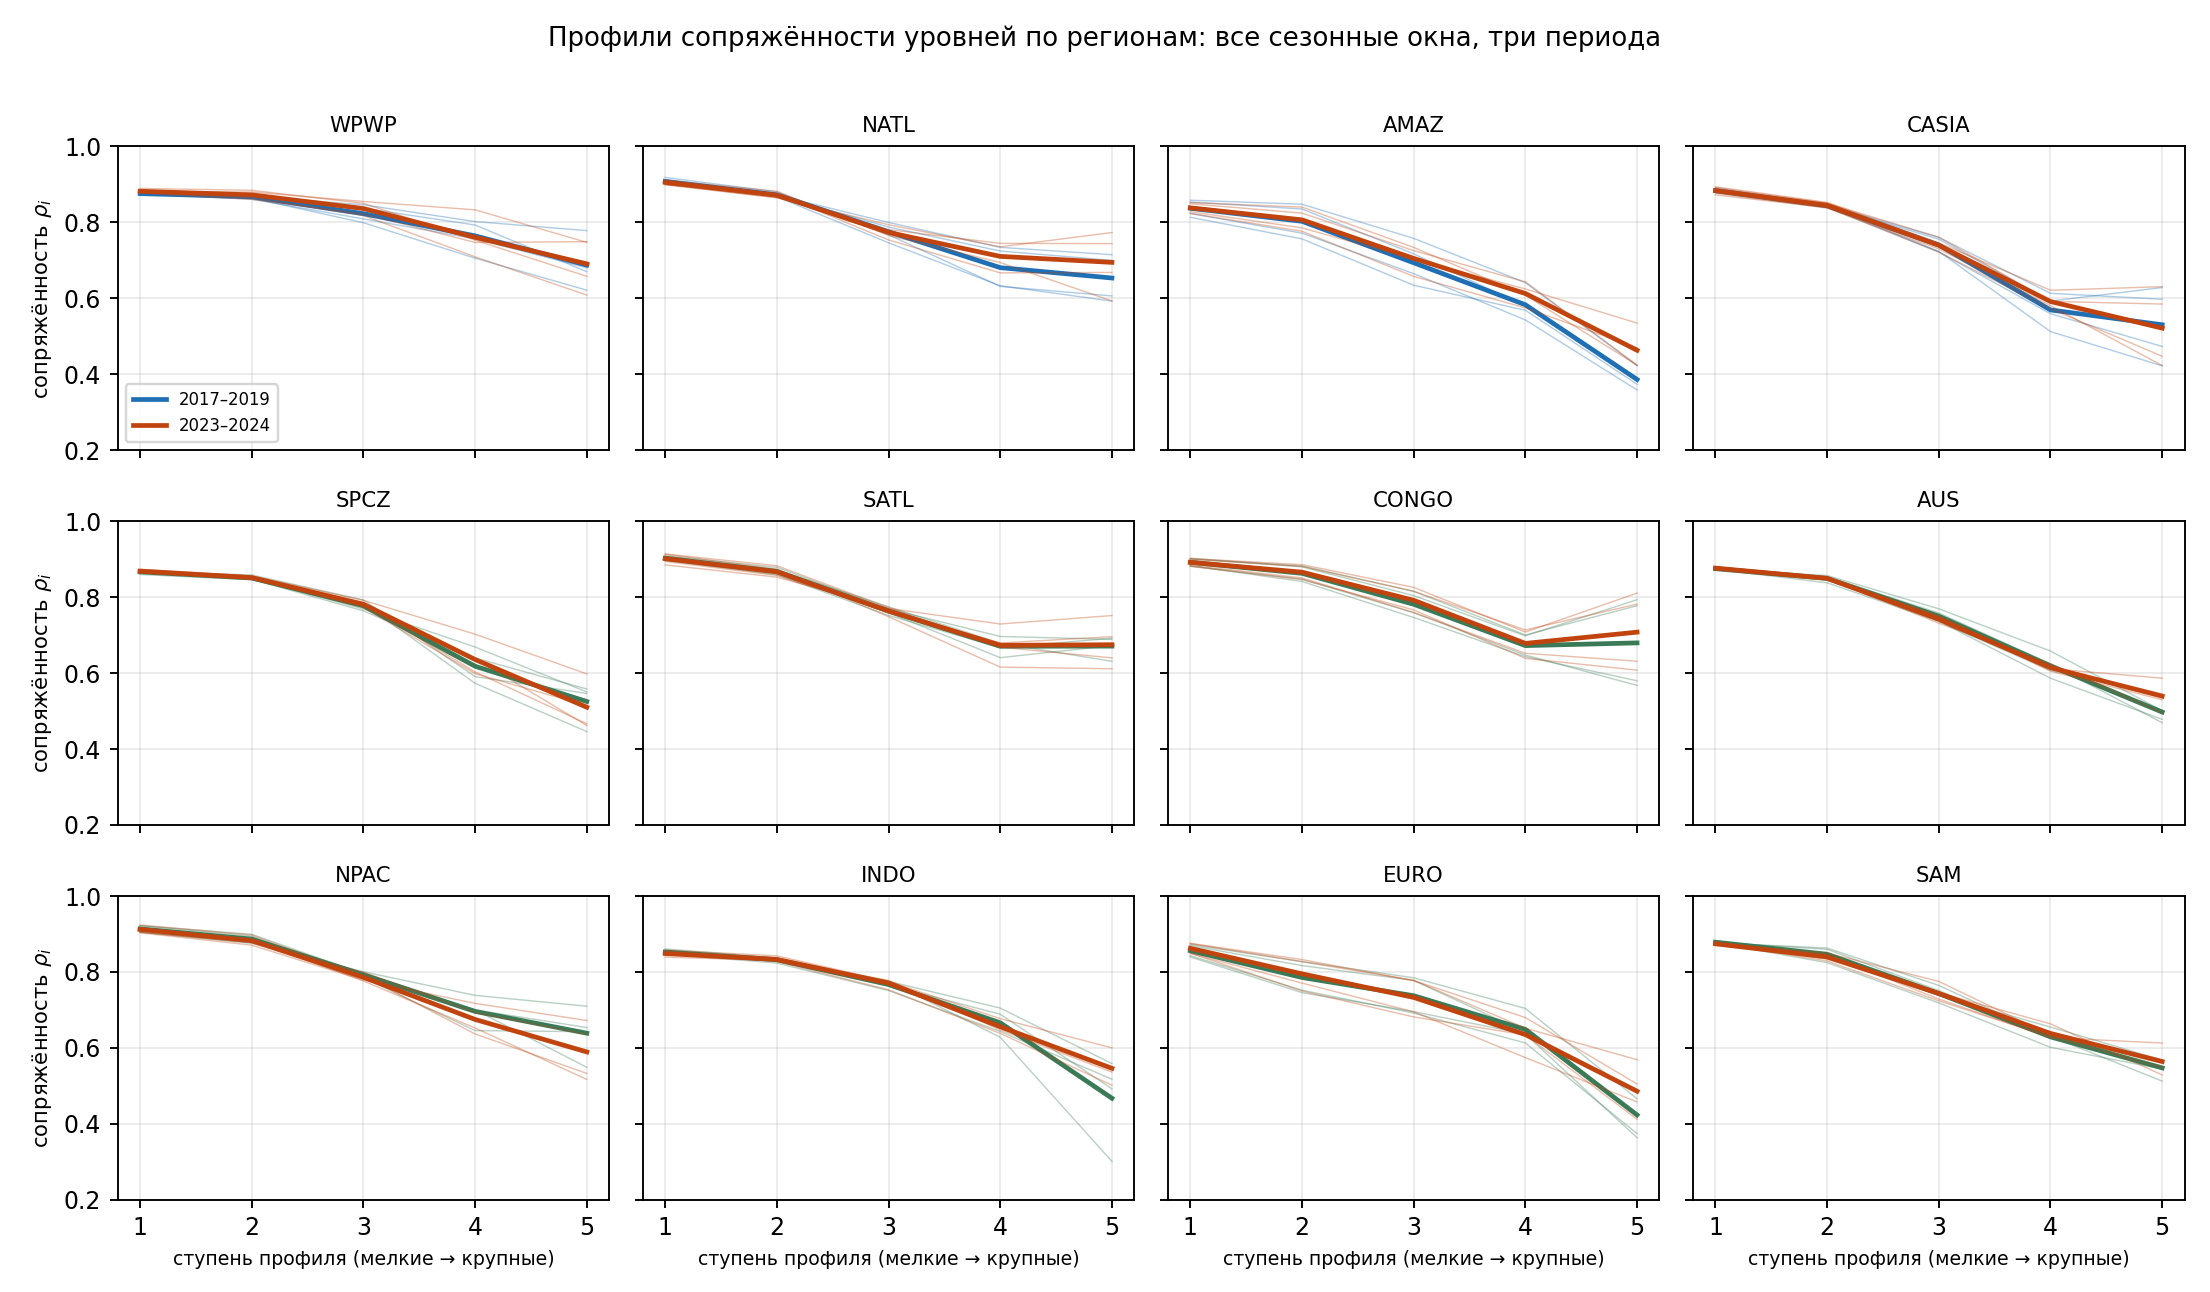
\includegraphics[width=\linewidth]{figures/article1/fig1_profiles.png}

\noindent Рис. 1. Профили сопряженности уровней $P$ для двенадцати основных областей (коды -- табл. 1): тонкие линии -- отдельные сезонные окна, жирные -- средние по периодам 2017--2019, 2021--2022 и 2023--2024 гг. Ступени 1--5 отвечают парам соседних уровней от (мельче 50; 50--100 км) до (400--800; 800--1600 км).

\clearpage
\noindent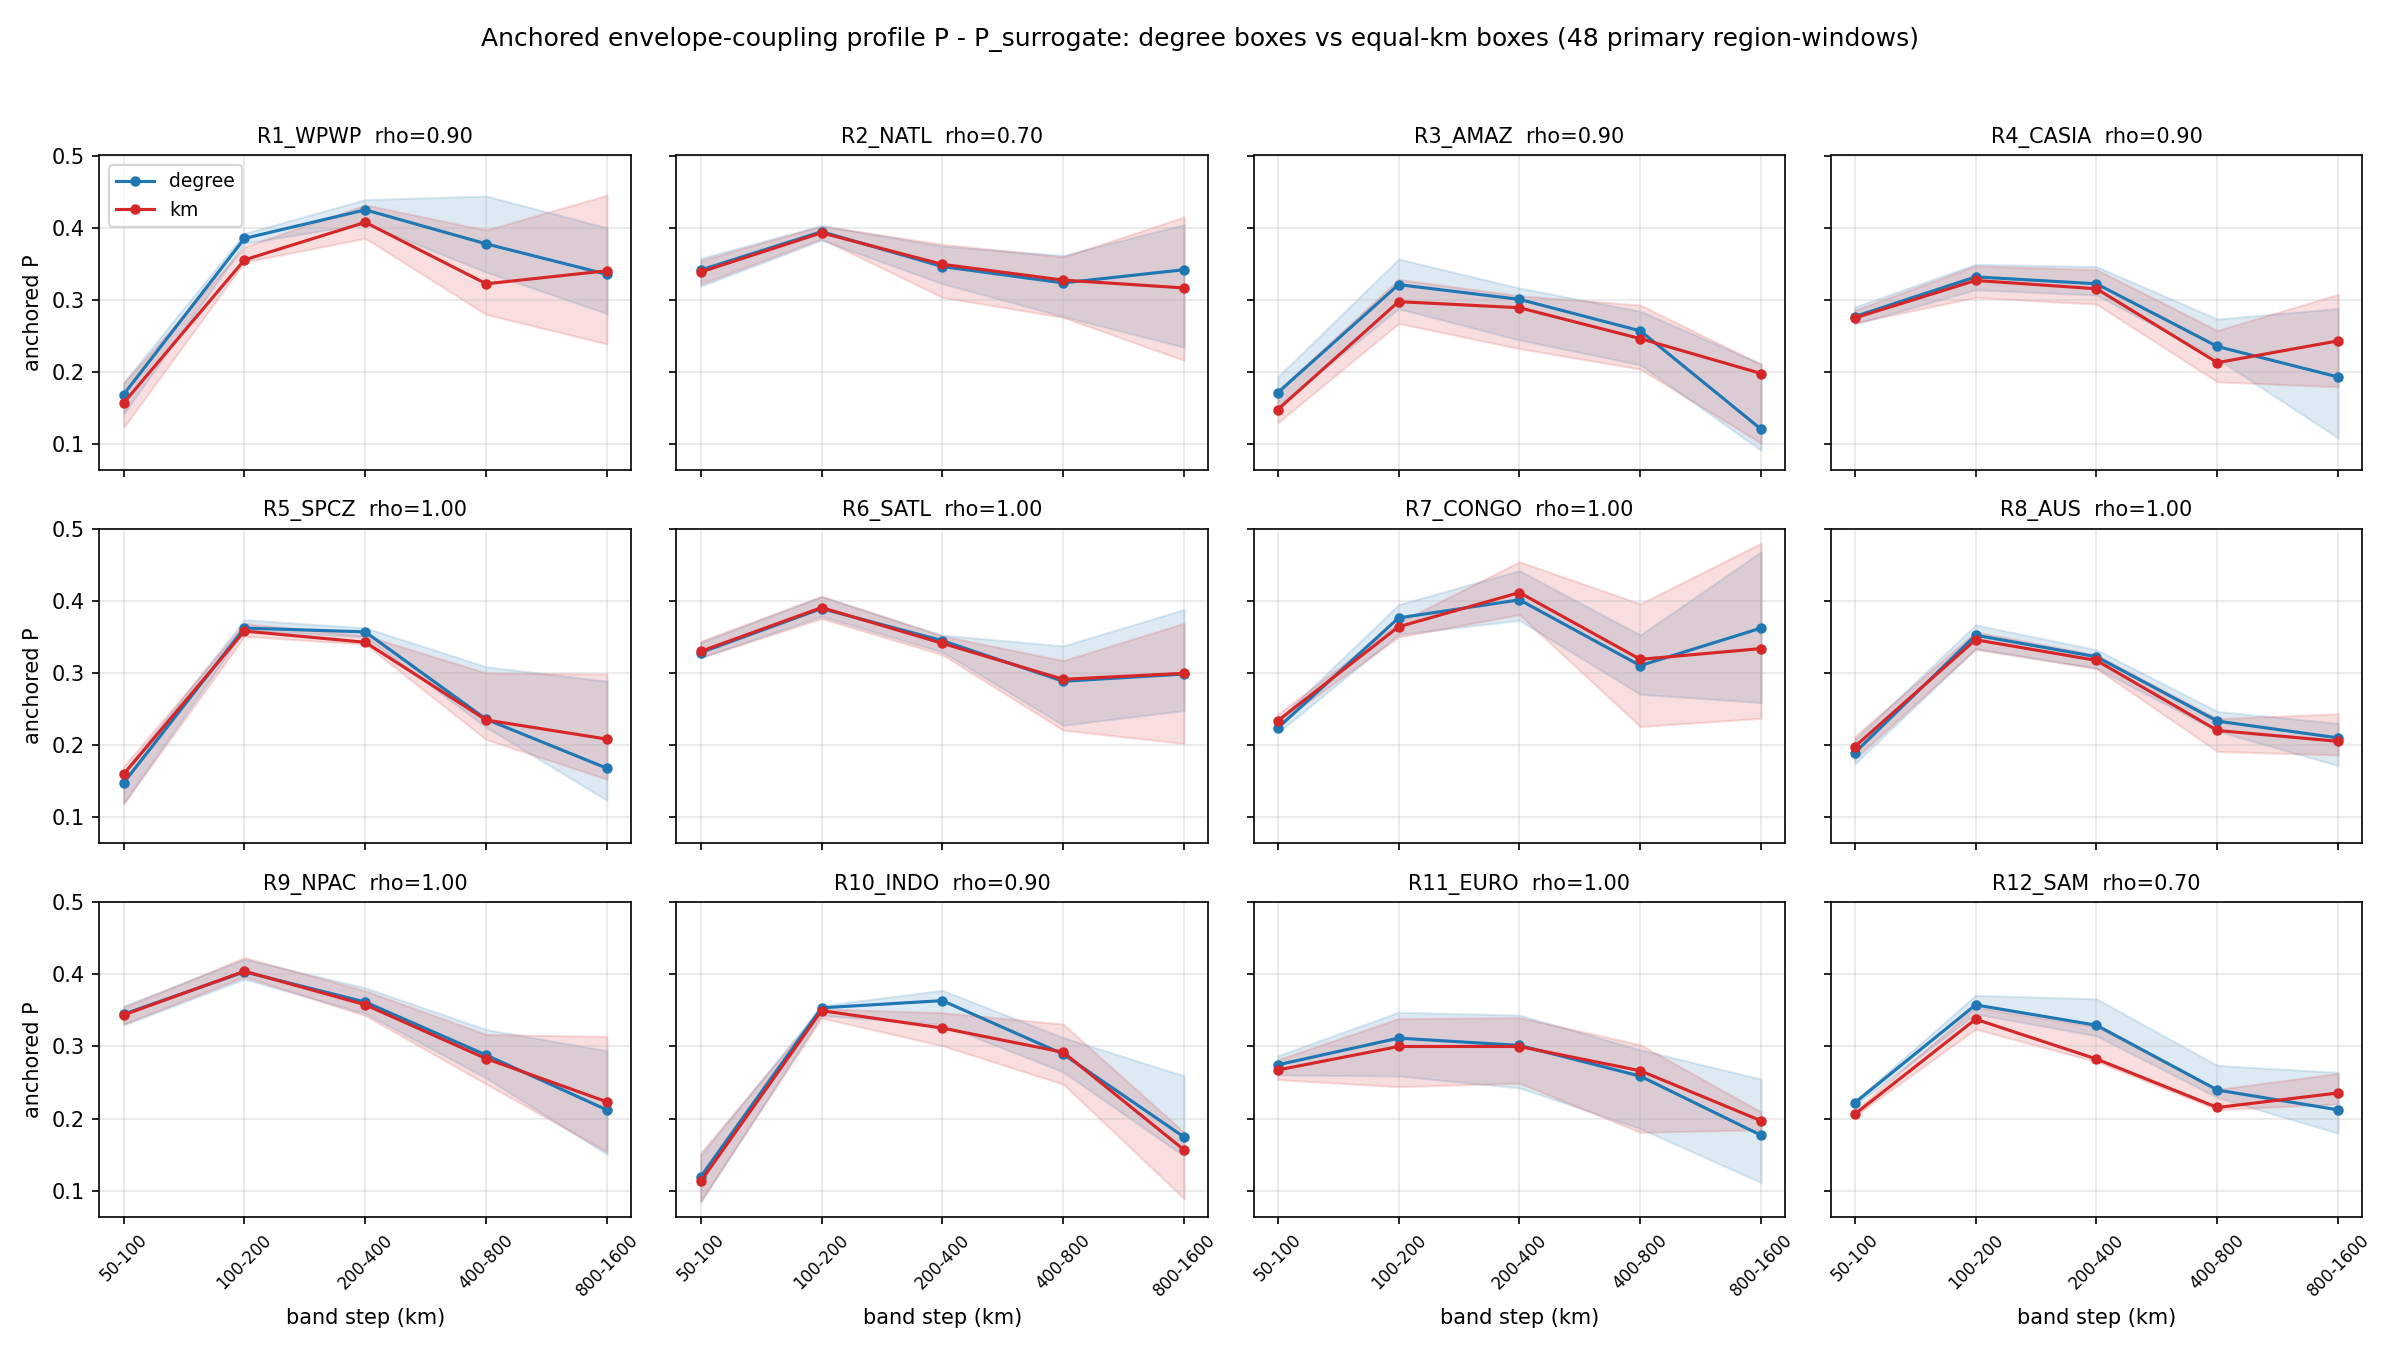
\includegraphics[width=\linewidth]{figures/article1/fig3_geometry.png}

\noindent Рис. 2. Контроль геометрии построением выборки: профили сопряженности с суррогатной поправкой $P - \Psurr$ на градусных областях $20^\circ \times 40^\circ$ (синий, “degree”) и на равновеликих областях $2000 \times 2800$ км (красный, “km”) для двенадцати регионов, 48 основных регион-окон 2023--2024 гг. Полосы -- размах по окнам; в заголовках панелей -- ранговая корреляция профилей двух нарезок по региону; по оси абсцисс -- полосы ступеней, км.

\clearpage
\noindent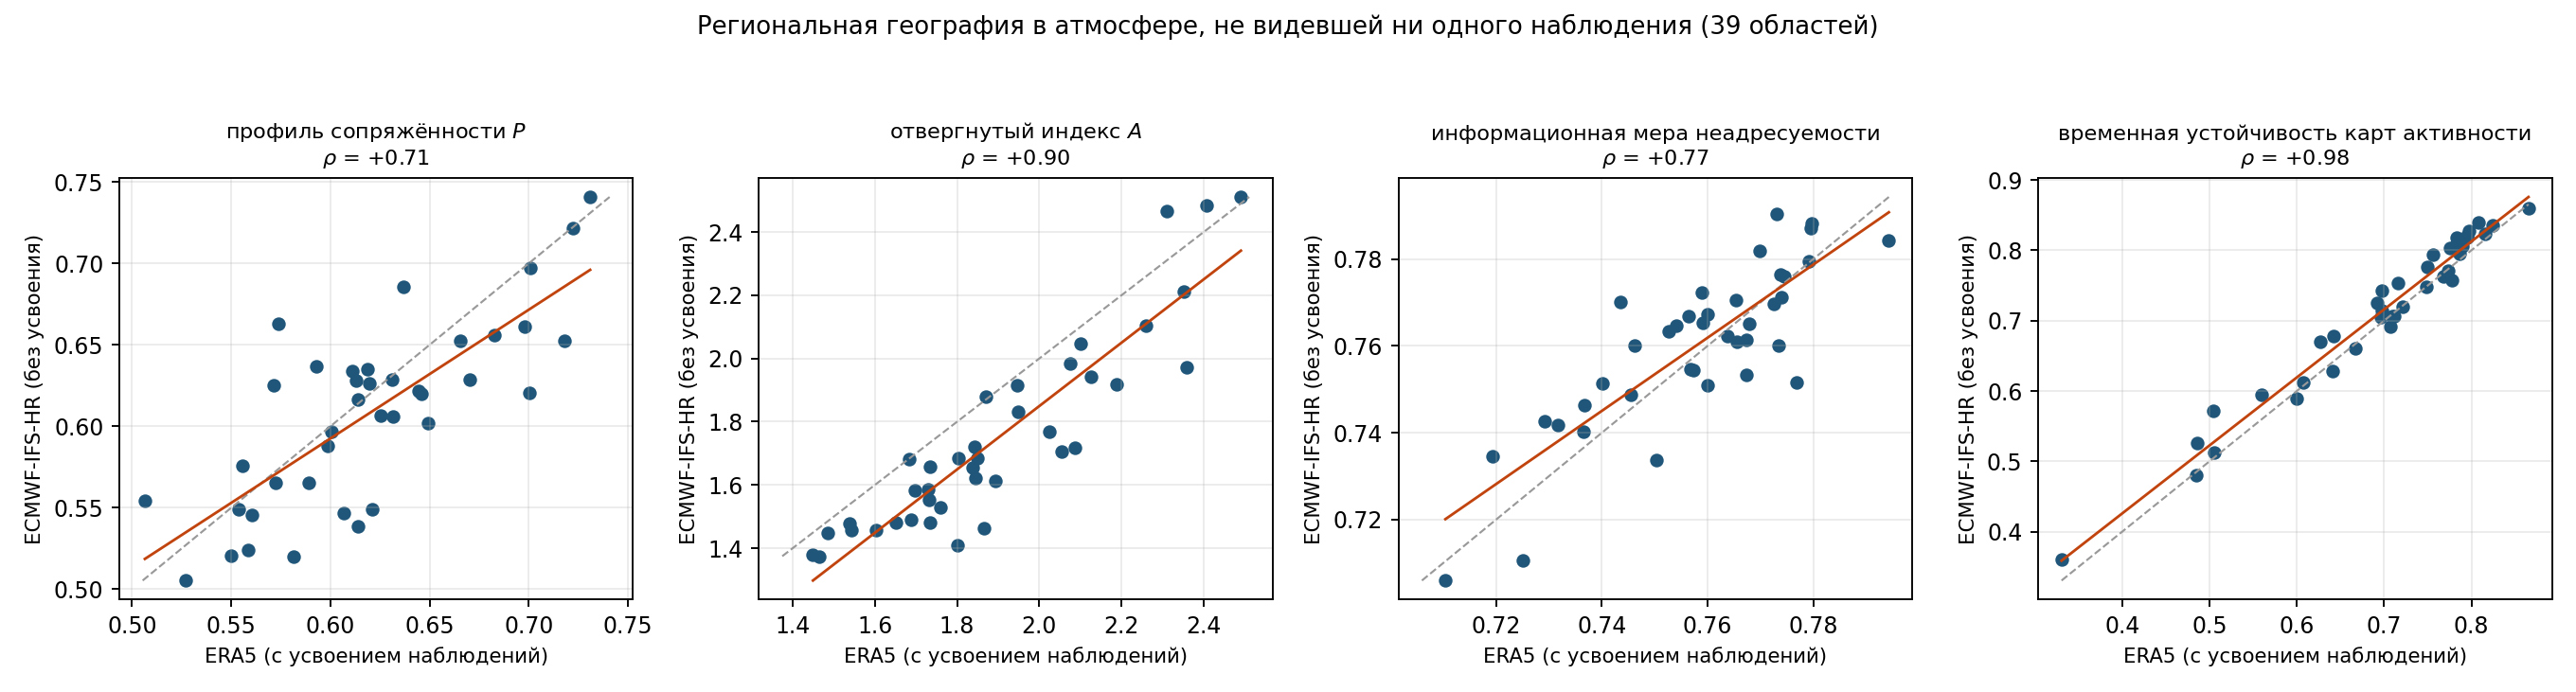
\includegraphics[width=\linewidth]{figures/article1/fig4_free_running.png}

\noindent Рис. 3. Сопоставление региональной географии по ERA5 (ось абсцисс) и по свободному расчету ECMWF-IFS-HR без усвоения наблюдений (ось ординат) для 39 областей. Слева направо: профиль сопряженности $P$; отвергнутый индекс невзаимности $A$ (показан для полноты: воспроизводимость индекса не оспаривается, отвергнуто его истолкование); независимая информационная мера межуровневой связи; временная устойчивость карт активности. Пунктир -- линия равенства.

\clearpage
\noindent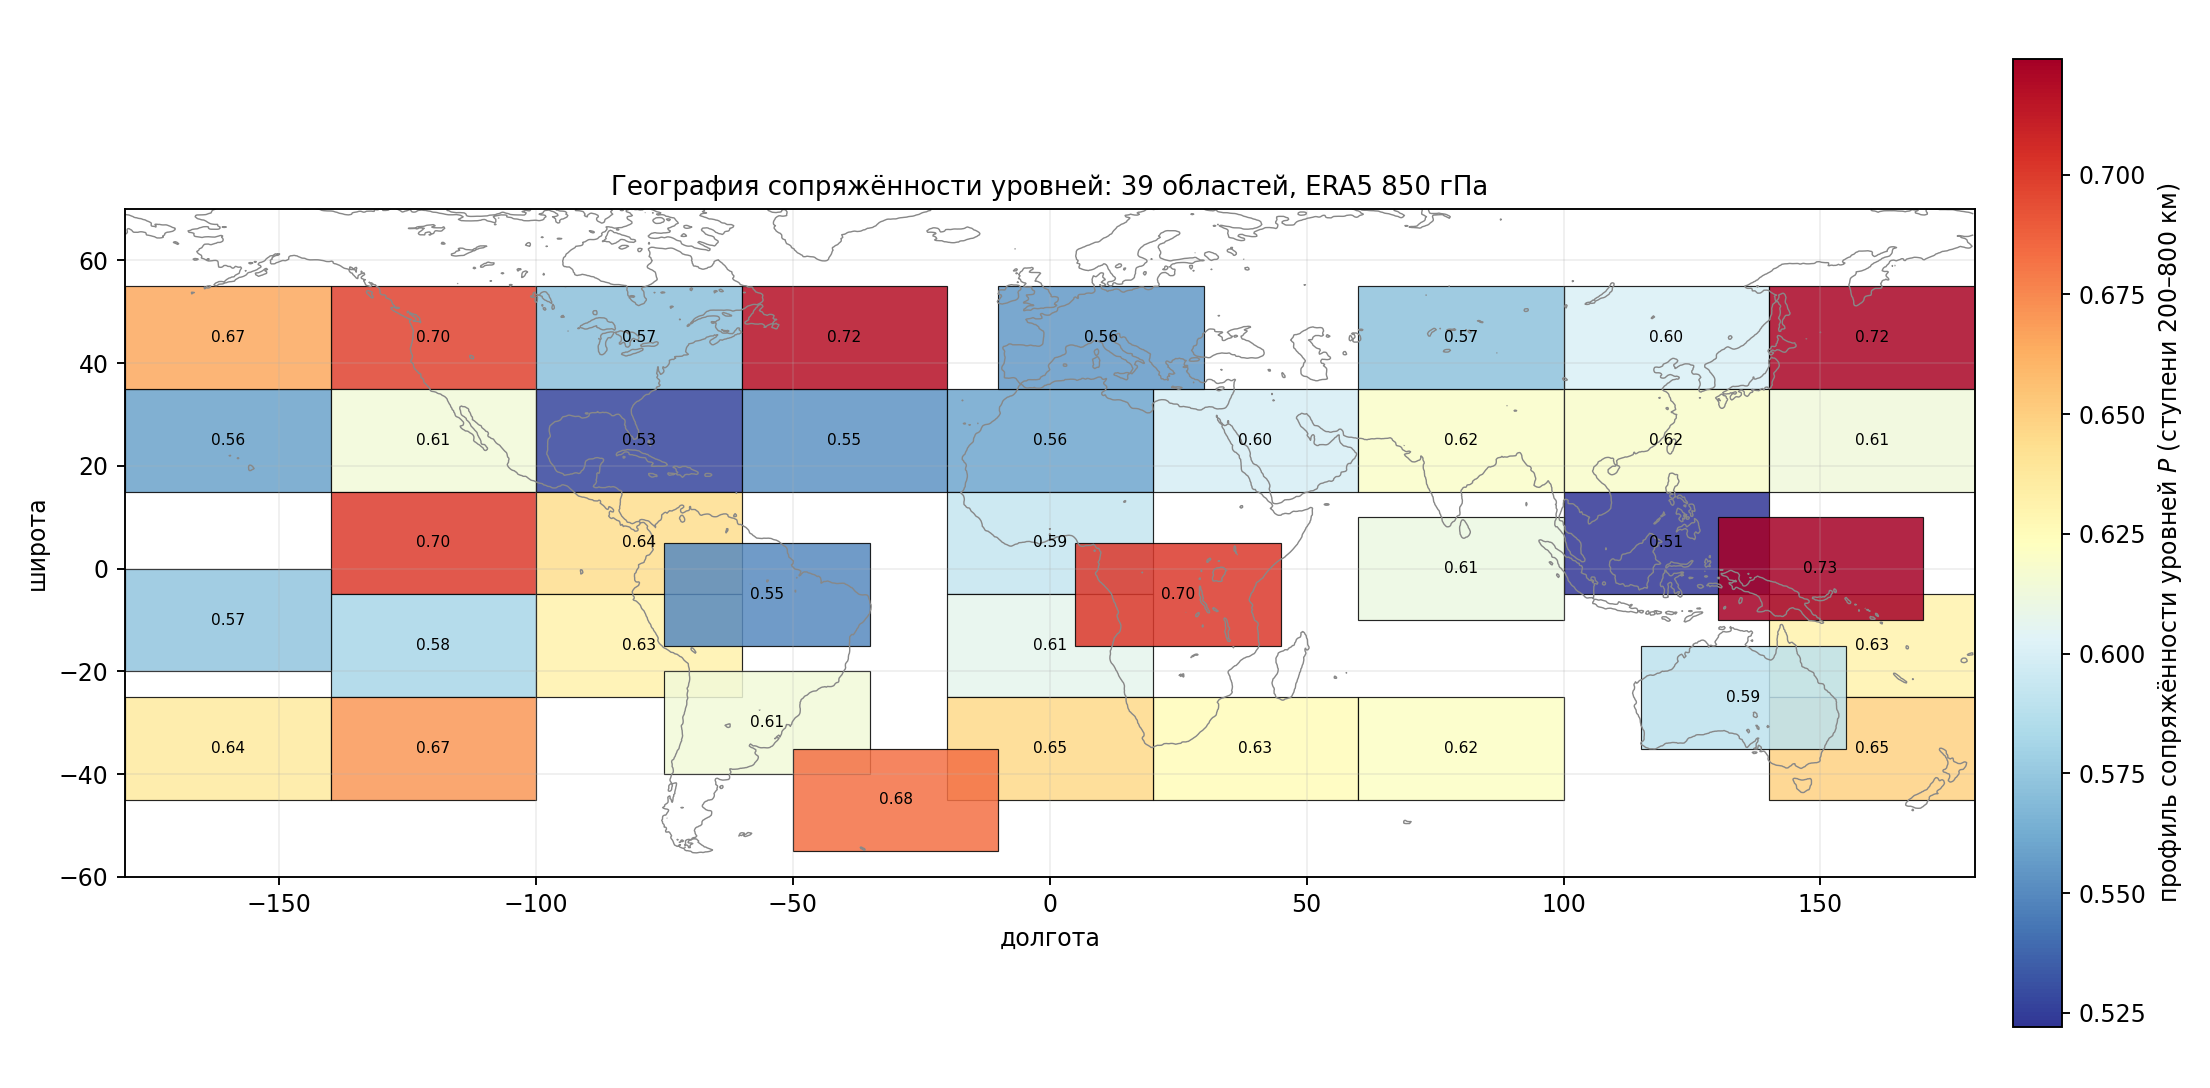
\includegraphics[width=\linewidth]{figures/article1/fig2_map.png}

\noindent Рис. 4. География сопряженности уровней: средние значения профиля по разрешенным ступеням 4--5 (пары полос 200--400/400--800 и 400--800/800--1600 км) для 39 областей, ERA5, 850 гПа; окна 2023--2024 гг. (решеточные области -- 2024 г.). Двенадцать областей выбраны содержательно, 27 -- формальным решеточным правилом.

\clearpage
\noindent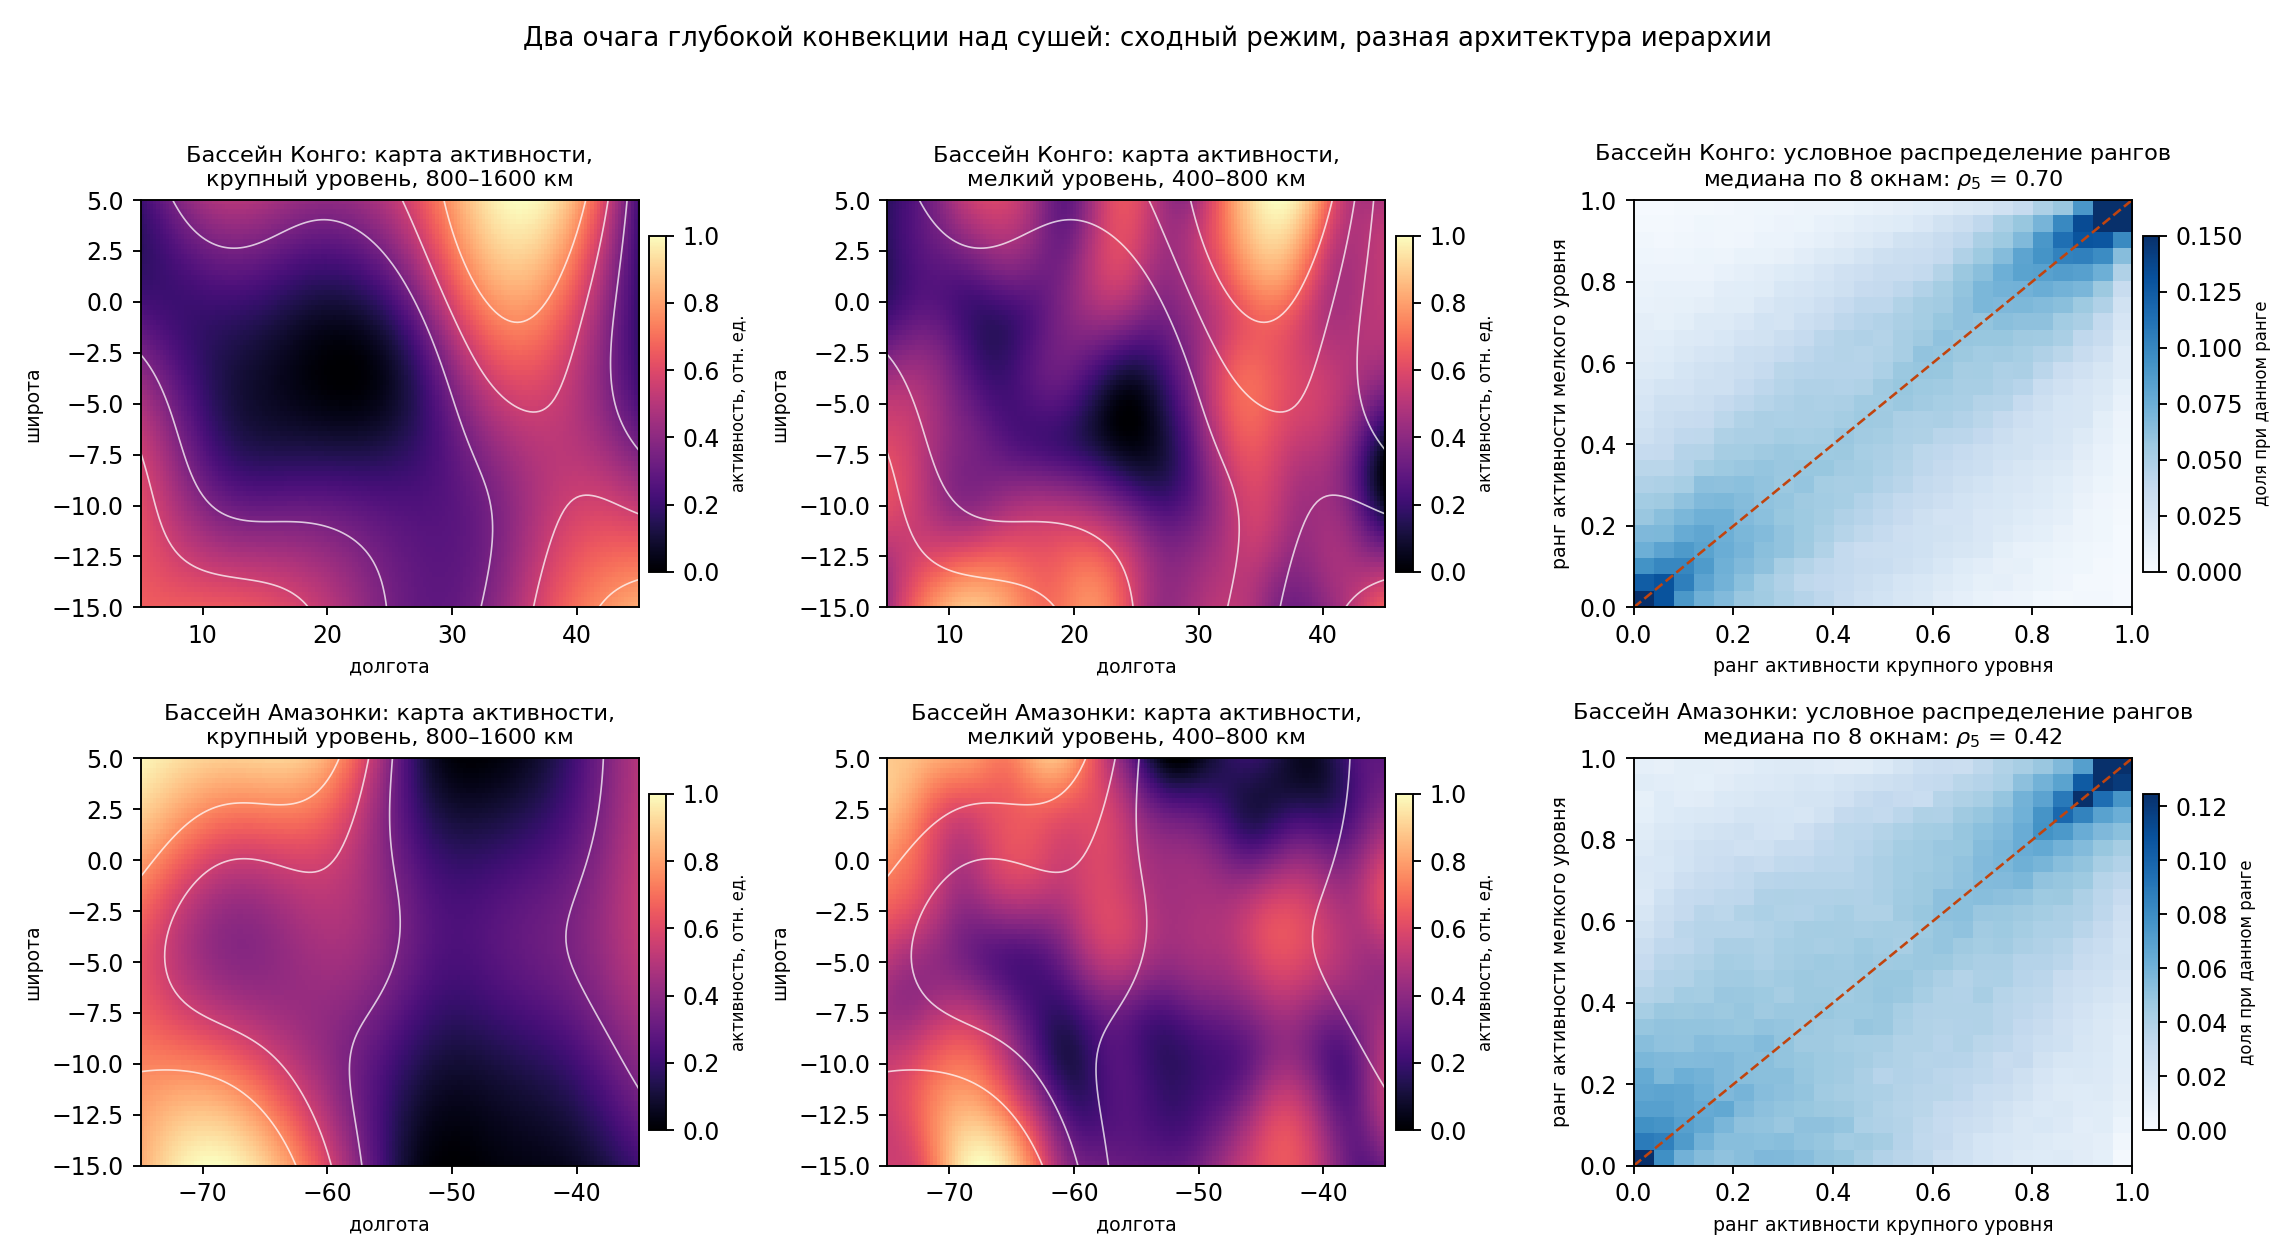
\includegraphics[width=\linewidth]{figures/article1/fig5_congo_amazon.png}

\noindent Рис. 5. Бассейны Конго (вверху) и Амазонки (внизу), январь--март 2023 г. Слева и в центре -- карты активности крупного (800--1600 км) и мелкого (400--800 км) уровней на один срок; белые изолинии -- активность крупного уровня, одни и те же на обеих картах ряда. Справа -- совместное распределение пространственных рангов активности двух уровней по всем срокам окна; пунктир -- диагональ полного соответствия. В Конго мезомасштабная активность привязана к крупному полю, в Амазонии -- нет.

\clearpage
\begin{center}
{\large\bfseries Coupling of hierarchical levels of the atmospheric circulation as a regional invariant}

\medskip
{\bfseries N. S. Sotiriadi\textsuperscript{*}}

Independent researcher, [City], Russia

\textsuperscript{*}E-mail: n.sotiriadi@gmail.com
\end{center}

\begin{singlespace}
\noindent\textbf{Abstract.} Spectral and fractal analysis of geographical fields answers the question of the scales at which the levels of organisation of a geosystem are located. The next question concerns the relation between levels: is the placement of mesoscale variability predetermined by the adjacent large level, or does it settle for local reasons of its own? Using the relative-vorticity field at 850 hPa (ERA5 reanalysis, 2017--2024; 12 main and 27 control regions) we construct a measure of this relation, the coupling profile of adjacent octave levels $P$: the spatial correlation of the activity maps of two adjacent scales, corrected for the contribution of the decomposition procedure itself. We test the hypothesis that the profile is a regional invariant in the operational sense: it keeps its value under a change of season, year, ENSO phase, data source and partition of the territory, while distinguishing circulation regimes. The hypothesis is confirmed on samples that did not take part in constructing the quantity ($p = 0.001$). Four alternative explanations -- numerical dissipation of the reanalysis, the power spectrum of the field, the geometry of the latitude--longitude grid and the observing network -- are tested by direct controls: the regional signature survives restriction to resolved steps, carries reproducible information beyond the spectrum (equal-area control: $p = 0.033$), is reproduced under an equal-area partition and in a free-running model integration that assimilates no atmospheric observations (rank correlation 0.71 against an internal ceiling of 0.93). Higher values belong to the extratropical storm tracks, lower values to moist-convective regimes; the Congo and Amazon basins, similar in standard regime characteristics, differ in the architecture of their hierarchy. The quantity adds to the toolkit of regionalisation a characteristic of the structure of inter-level relations; its limits of applicability, including rejected interpretations, are stated explicitly.

\smallskip
\noindent\textbf{Keywords:} hierarchical organisation of geosystems, invariants of a dynamic geosystem, scale, mesoscale variability, storm tracks, deep convection, reanalysis, regionalisation, falsification design.

\smallskip
\noindent\textbf{Funding.} The study received no external funding. The author declares no conflict of interest.
\end{singlespace}

\end{document}
